\title{Funções: passagem de parâmetros}
\frame{\maketitle}

\begin{frame}{Terminologia: Kernighan \& Ritchie}

\small

\begin{description}
\item[Parâmetro:] é uma variável definida em uma definição de função
ou uma declaração de protótipo de função. Exemplo:

{\tt  int soma(int x, int y);}

\bigskip

{\tt x} e {\tt y} são parâmetros.

\pause
\item[Argumento:] é um valor usado em uma chamada para
função. Exemplo: \\

{\tt  s = soma(x, y);}
\bigskip
{\tt x} e {\tt y} são argumentos.
\end{description}

\end{frame}

%% Extraído de Harbison/Steele's C Reference Manual
\begin{frame}[fragile]{Convenções de passagem de parâmetros}

 \CEE\ fornece somente \alert{chamadas por valor} na passagem de
 parâmetros~\cite{cref2002}.

  \begin{lstlisting}
    /* troca os valores de x e y */
    /* versão INCORRETA */
    void troca_err(int x, int y) 
    {
      int tmp;
      
      tmp = x; 
      x = y; 
      y = tmp;
    }
    
    void main()
    {
      int a = 3;
      int b = 8
      troca_err(a,b); }/* FALHA para trocar a e b */
    }
\end{lstlisting}
\end{frame}

\begin{frame}[fragile]{Convenções de passagem de parâmetros, cont.}
  \begin{lstlisting}
    /* troca os valores de x e y */
    /* versão CORRETA */
    void troca(int *x, int *y) 
    {
      int tmp;
      
      tmp = *x; 
      *x = *y; 
      *y = tmp;
    }
    
    void main()
    {
      int a = 3;
      int b = 8
      troca(&a, &b);  /* Troca de conteúdo entre a e b */
    }
\end{lstlisting}
\end{frame}


\begin{frame}[fragile]{Definições equivalentes}

\CEE\ permite passar por valor somente variáveis ``atômicas''.

\begin{lstlisting}
/* equivalentes */
func(int *v) {...} 
func(int v[ ]) {...}
func(int v[200]) {...}
\end{lstlisting}

\bigskip
\pause

%%% Local Variables:
%%% mode: latex
%%% TeX-master: t
%%% End:


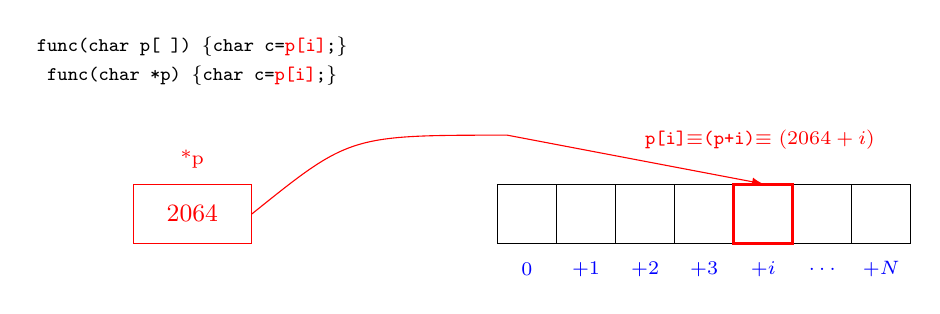
\begin{tikzpicture}

\def\offset{.75cm}
\def\addr{2064}

\tikzset{
        every node/.style={font=\scriptsize},
        every path/.style={->,>=latex,draw},
        data/.style={minimum height=.75cm, draw},
        pointer/.style={data,font=\small,red,minimum width=2*\offset},
        array/.style={data,minimum width=\offset},
        index/.style={blue}
}

\node[pointer] (P) at (0,0) {2064};
\node[red] (pointer label) [above of=P,yshift=-\offset/2.5] {*p};

\node (MEM) [right of=P,xshift=3*\offset] {};

\foreach \i/\l in {0/0,1/+1,2/+2,3/+3,4/+$i$,5/$\ldots$,6/+$N$} {
     \node[array] (A\i) [right of=MEM,xshift=\i*\offset] {};
     \node[index] [below of=A\i,yshift=\offset/2.5] {\l};
}

\draw[red] (P.east) .. controls (2,1) .. (4,1)  --  node[above
right,red] {\tt p[i]$\equiv$(p+i)$\equiv(2064+i)$}  (A4.north);

\node[array,red, very thick] at (A4) {};

\node [above of=P,yshift=1.5*\offset] {\tt func(char p[ ]) \{char c={\color{red}p[i]};\}};
\node [above of=P,yshift=\offset] {\tt func(char *p) \{char c={\color{red}p[i]};\}};

\end{tikzpicture}


\end{frame}

\begin{frame}[fragile]{Usos comuns de \alert{vetor/ponteiro} como parâmetro}

\begin{lstlisting}
int nat; /*  ``atomica'' */
int *nat_ptr; /* ponteiro */
int nat_vet[10]; /* vetor */
\end{lstlisting}

\bigskip
\scriptsize\noindent
\begin{tabular}[h]{lll}\hline
\bf \scriptsize Argumento  & \bf Tipo & \bf Propósito \\\hline
\color{blue}{\tt func(\&nat);} & \color{blue}endereço de um inteiro & \color{blue}Para ``passagem por
 \\
& &\color{blue} referência'' de um inteiro \\
\color{green!30!black}{\tt func(nat\_ptr);} & \color{green!30!black}ponteiro para inteiro & \color{green!30!black}Para passar um ponteiro \\
\color{blue}{\tt func(nat\_vet);} & \color{blue}vetor de inteiros & \color{blue}Para passar um vetor \\
\color{green!30!black}{\tt func(\&nat\_vet[i]);} & \color{green!30!black}endereço de um elemento do vetor & \color{green!30!black}Para passar
uma fatia \\
&& \color{green!30!black}do vetor \\
\\\hline 
\end{tabular}

\end{frame}

\begin{frame}[fragile]{Vetores como argumentos: operações válidas, cont.}
\begin{lstlisting}
/* Ponteiros e vetores. */
int vetor1[100], vetor2[200];

/* Ponteiro como argumento */
void fun_p(int *pt) {
  pt = vetor1; /* OK */
}
\end{lstlisting}
\end{frame}

\begin{frame}[fragile]{Vetores como argumentos: operações válidas, cont.}
  \begin{lstlisting}
    /* Ponteiros e vetores. */
    int vetor1[100], vetor2[200];

    /* Vetor como argumento */
    void fun_v(int v[ ]) {
      v = vetor2; /* OK */
    }
 \end{lstlisting}
\end{frame}

\begin{frame}[fragile]{Vetores como argumentos: operações válidas, cont.}

  {\scriptsize Como os vetores não foram passados como argumentos,
    ocorre \alert{FALHA} nas atribuições, pois os vetores não foram
    convertidos para ``ponteiros''. Ocorre erro nas tentativas de
    acesso às variáveis globais e atribuição de endereços a inteiros, pois
    {\tt vetor1 e vetor2} não são parametros da função.}
\begin{lstlisting}
/* Ponteiros e vetores. */
int vetor1[100], vetor2[200];

int main(int argc, char **argv) {
    int v[100];

    /* FALHA, tentativa de atribuir endereço aos vetores */
    v = vetor1;
    vetor1 = vetor2; 
    vetor2 = v;

    return 0;
}
\end{lstlisting}

\end{frame}

\begin{frame}{Leitura adicional}

\begin{thebibliography}{5}
\bibitem[Kernighan \& Ritchie, 1989]{C:1989}
    Brian W.\ Kernighan \& Dennis M.\ Ritchie.
    \newblock {\it \href{http://bit.ly/1byOUG6}{\CEE: A Linguagem de Programação, Padrão ANSI}.\/}
    \newblock Editora Campus, 2$^{a.}$\ edição, 1989.

\bibitem[Linden, 1994]{linden1994}
     Peter van der Linden.
     \newblock {\it \href{http://amzn.to/16j5Hgx}{Expert \CEE\ Programming: Deep \CEE\ Secrets}.\/}
     \newblock Prentice Hall, 1$^{st}$ edition, 1994.

\bibitem[Harbison III \& Steele Jr., 2002]{cref2002}
        Samuel P.\ Harbison \& Guy L.\ Steele Jr.
        \newblock {\it \CEE: A Reference Manual\/}.
        \newblock Prentice Hall, 5$^{th}$ edition, 2002.
\end{thebibliography}

\end{frame}
